% Define the top matter
\renewcommand{\moduleTitle}{Data Quality}
\renewcommand{\moduleAuthors}{%
  Sonika Tyagi \mailto{sonika.tyagi@agrf.org.au}
} \renewcommand{\moduleContributions}{%
  Nathan S. Watson-Haigh \mailto{nathan.watson-haigh@awri.com.au}%
}

%  Start: Module Title Page
\chapterstyle{module}
\chapter{\moduleTitle}
\newpage
% End: Module Title Page

\section{Key Learning Outcomes}

After completing this practical the user should be able to:
\item \\
\item \\
\item \\

\section{Resources You'll be Using}
Although we have provided you with an environment which contains all the tools
and data you will be using in this module, you may like to know where we have
sourced those tools and data from.
 
\subsection{Tools Used}
\begin{description}[style=multiline,labelindent=0cm,align=left,leftmargin=0.5cm]
  \item[FastQC]\hfill\\
  	\url{http://www.bioinformatics.babraham.ac.uk/projects/fastqc/}
  \item[fastx-toolkit]\hfill\\
  	\url{http://hannonlab.cshl.edu/fastx_toolkit/}
  \item[picard]\hfill\\
  	\url{http://picard.sourceforge.net/}
  \item[fastqmcf]\hfill\\
  	\url{http://code.google.com/p/ea-utils/wiki/FastqMcf}
\end{description}

\subsection{Sources of Data}
N/A


\newpage

\section{Introduction}

\begin{note}
Going on a blind date with your read set? For a better understanding of the
consequences please check the data quality!
\end{note}

For the purpose of this tutorial we are focusing only on the Illumina sequencing
which uses 'sequence by synthesis' technology in a highly parallel fashion.
Although Illumina high throughput  sequencing provides highly accurate sequence
data, several sequence artefacts, including base calling errors and small
insertions/deletions, poor quality reads and primer/adapter contamination are
quite common in the high throughput sequencing data. The primary errors are
substitution errors. The error rates can vary from 0.5-2.0\% with errors mainly
rising in frequency at the 3' ends of reads.

One way to investigate sequence data quality is to visualize the quality scores
and other metrics in a compact manner to get an idea about the quality of a read
data set. Read data sets can be improved by post processing in different ways
like trimming off low quality bases, cleaning up the sequencing adapters if any,
removing PCR duplicates if required. We can also look at other statistics such
as, sequence length distribution, base composition, sequence complexity,
presence of ambiguous bases etc. to assess the overall quality of the data set.
Highly redundant coverage (>15X) of the genome can be used to correct sequencing
errors in the reads before assembly and errors. Various k-mer based error
correction methods exist but are beyond the scope of this tutorial.

\section{Prepare the Environment}

\being{information}
To investigate sequence data quality we would demonstrate tools called FastQC
and fastx-toolkit. FastQC will process and present the reports in visual manner.
Based on the results the sequence data can be processed using the fastx-toolkit.
We will use one data set in this practical, which can be found in the QC
directory on your desktop.
\end{information}

\begin{steps}
Open the Terminal and go to the right directory where the data are stored:
\begin{lstlisting}
cd ~/QC/
pwd
\end{lstlisting}

At any time help can be displayed for 'fastqc' program with the following command:
\begin{lstlisting}
fastqc -h
\end{lstlisting}

\end{steps}


\section{Quality Visualisation}

\begin{information}
We have file for a good quality and bad quality statistics. On executing the
FastQC commands above, it will generate a zipped and unzipped folder for each
input file.
\end{information}

\begin{steps}
Execute the following command on the two files:
\begin{lstlisting}
fastqc -f fastq bad_example.fastq 
fastqc -f fastq good_example.fastq
\end{lstlisting}

View the FastQC report files 'fastqc\_report.html', using a web browser such as
firefox, to see examples of a bad quality data.

\begin{lstlisting}
firefox bad_example_fastqc/fastqc_report.html &
\end{lstlisting}

\end{steps}

\begin{note}
The report file will have a Basic Statistics table and various graphs and tables
for different quality statistics. E.g.:
\end{note}

% Table generated by Excel2LaTeX from sheet 'Sheet1'
\begin{table}[H]
  \centering
  \caption{FastQC Basic Statistics table}
    \begin{tabular}{ll}
    \toprule
    Filename & bad\_example.fastq \\
    \midrule
    File type & Conventional base calls \\
    Encoding & Sanger / Illumina 1.9 \\
    Total Sequences & 40000 \\
    Filtered Sequences & 0 \\
    Sequence length & 100 \\
    \%GC  & 48 \\
    \bottomrule
    \end{tabular}%
  \label{tab:badexampleuntrimmed}%
\end{table}%

\begin{figure}[H]
\centering
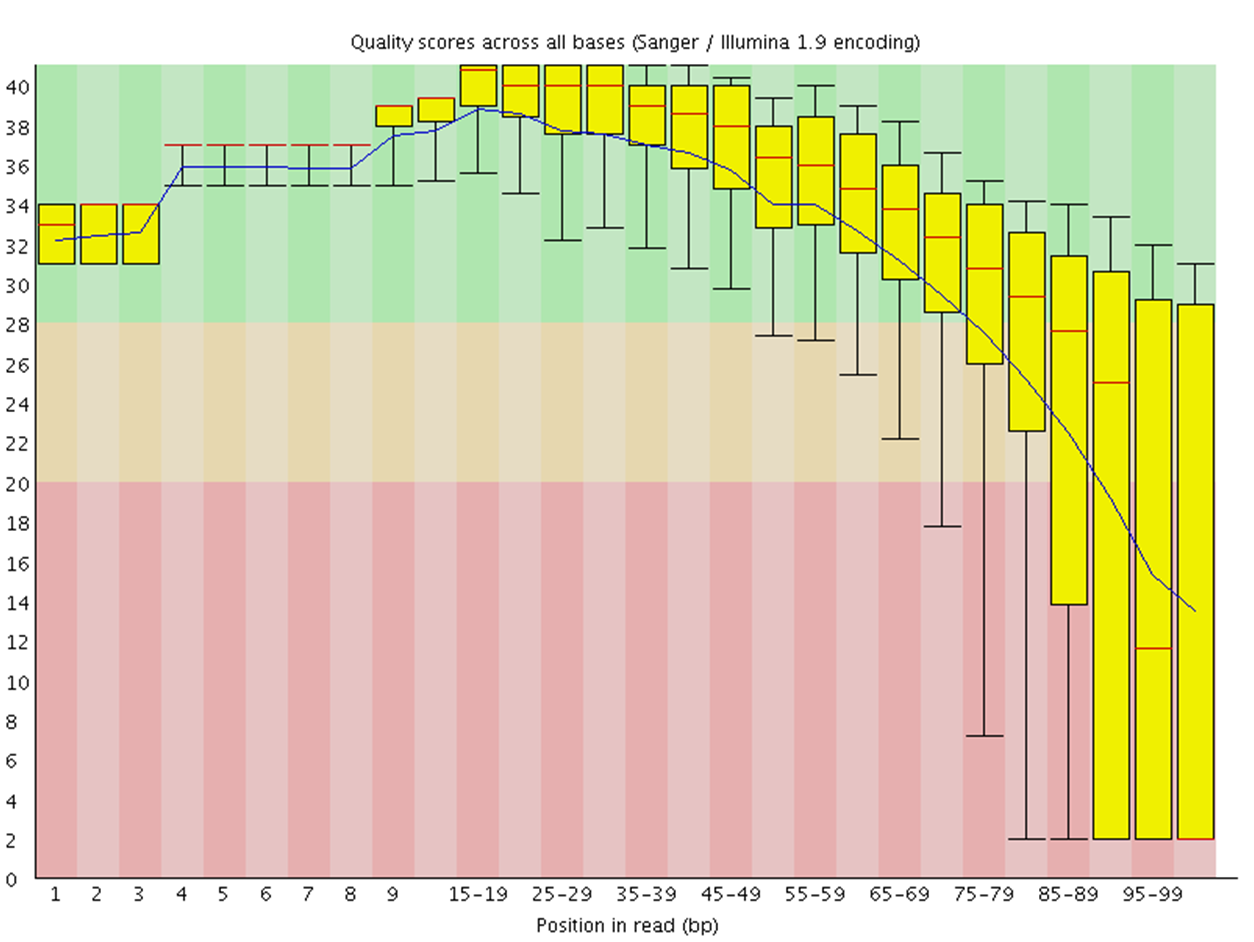
\includegraphics[width=0.8\textwidth]{ngs-qc/bad_example.png}
\caption{per base sequence quality plot: visual output from FastQC. Base positions in the reads are shown on x-axis and quality score (Q Score) are shown on the Y-axis}
\label{fig:bad_example_plot}
\end{figure}

\begin{information}
A quality score (or Q-score) expresses an error probability.  In particular, it
serves as a convenient and compact way to communicate very small error
probabilities.
Given an assertion, A, the probability that A is not true, P(~A), is expressed
by a quality score,Q(A), according to the relationship:

Q(A) =-10 log10(P($\sim$A))

where P($\sim$A) is the estimated probability of an assertion A being wrong.
The relationship between the quality score and error probability is demonstrated
with the following table:

% Table generated by Excel2LaTeX from sheet 'Sheet1'
\begin{table}[H]
  \centering
  \caption{Error probabilities associated with various quality (Q) values}
    \begin{tabular}{rr}
    \toprule
    \textbf{Quality score, Q(A)} & \textbf{Error probability, P($\sim$A)} \\
    \midrule
    10    & 0.1 \\
    20    & 0.01 \\
    30    & 0.001 \\
    40    & 0.0001 \\
    \bottomrule
    \end{tabular}%
  \label{tab:addlabel}%
\end{table}%

\end{information}

\begin{questions}
How many sequences were there in your file? What is the read length?

Does the quality score value vary throughout the read length?
(hint: look at the 'per base sequence quality plot')

What is the quality score range you see?

At around which position do the score start falling below Q20? 

Why does the quality deteriorate at the end of the read?

How can we trim the reads to filter out the low quality data?

\end{questions}

\begin{bonus}
\subsection{Good Quality Data}
View the FastQC report files fastqc\_report.html to see examples of a good
quality data and compare the quality plot with that of the bad\_example\_fastqc.

\begin{lstlisting}
firefox good_example_fastqc/fastqc_report.html &
\end{lstlisting}
\end{bonus}

\begin{note}
Sequencing errors can complicate the downstream analysis, which normally
requires that reads be aligned to each other (for genome assembly) or to a
reference genome (for detection of mutations). Sequence reads containing errors
may lead to ambiguous paths in the assembly or improper gaps. In variant
analysis projects sequence reads are aligned against the reference genome. The
errors in the reads may lead to more number of mismatches than expected due to
mutations alone. But if these errors can be removed or corrected, the reads
alignment and hence the variant detection will improve. The assemblies will also
improve after pre-processing the reads with errors.
\end{note}

\section{Read Trimming}
The read trimming can be done in a variety of different ways. Choose a method
which best suits your data. Here we are giving examples of fixed-  base trimming
and quality score-based trimming.

\subsection{Fixed Length Trimming}
Low quality read ends can be trimmed using a fix length timmer. We will use the
fastx\_trimmer from the fastx-toolkit. usage message to find out various options
you can use with this tool. Type \fontt{fastx_trimmer -h} at anytime to display help.

\begin{steps}
In order to do fixed trimming with the fastq file \texttt{bad\_example.fastq}
use the following command. The output will be stored in
\texttt{bad\_example\_trimmed01.fastq}.

\begin{lstlisting}
cd ~/QC
fastx_trimmer -h
fastx_trimmer -Q 33 -f 1 -l 80 -i bad_example.fastq -o bad_example_trimmed01.fastq
\end{lstlisting}
\end{steps}

\begin{note}
We used the following options in the command above:
\begin{description}[style=multiline,labelindent=0cm,align=right,leftmargin=5cm,font=\ttfamily]
 \item[-Q 33] Indicates the input quality scores are Phred+33 encoded
 \item[-f] First base to be retianed in the output
 \item[-l] Last base to be retained in the output
 \item[-i] Input fastq file name
 \item[-o] Output file name
\end{description}
\end{note}

\begin{steps}
Run fastqc on the trimmed file and visualise the quality scores of the trimmed file.
\begin{lstlisting}
fastqc -f fastq bad_example_trimmed01.fastq
firefox bad_example_trimmed01_fastqc/fastqc_report.html &
\end{lstlisting}

The output should look like:

\begin{table}[H]
  \centering
  \caption{FastQC Basic Statistics table}
    \begin{tabular}{ll}
    \toprule
    Filename & bad\_example\_trimmed01.fastq \\
    \midrule
    File type & Conventional base calls \\
    Encoding & Sanger / Illumina 1.9 \\
    Total Sequences & 40000 \\
    Filtered Sequences & 0 \\
    Sequence length & 80 \\
    \%GC  & 48 \\
    \bottomrule
    \end{tabular}%
  \label{tab:badexampletrimmed}%
\end{table}%

\begin{figure}[H]
\centering
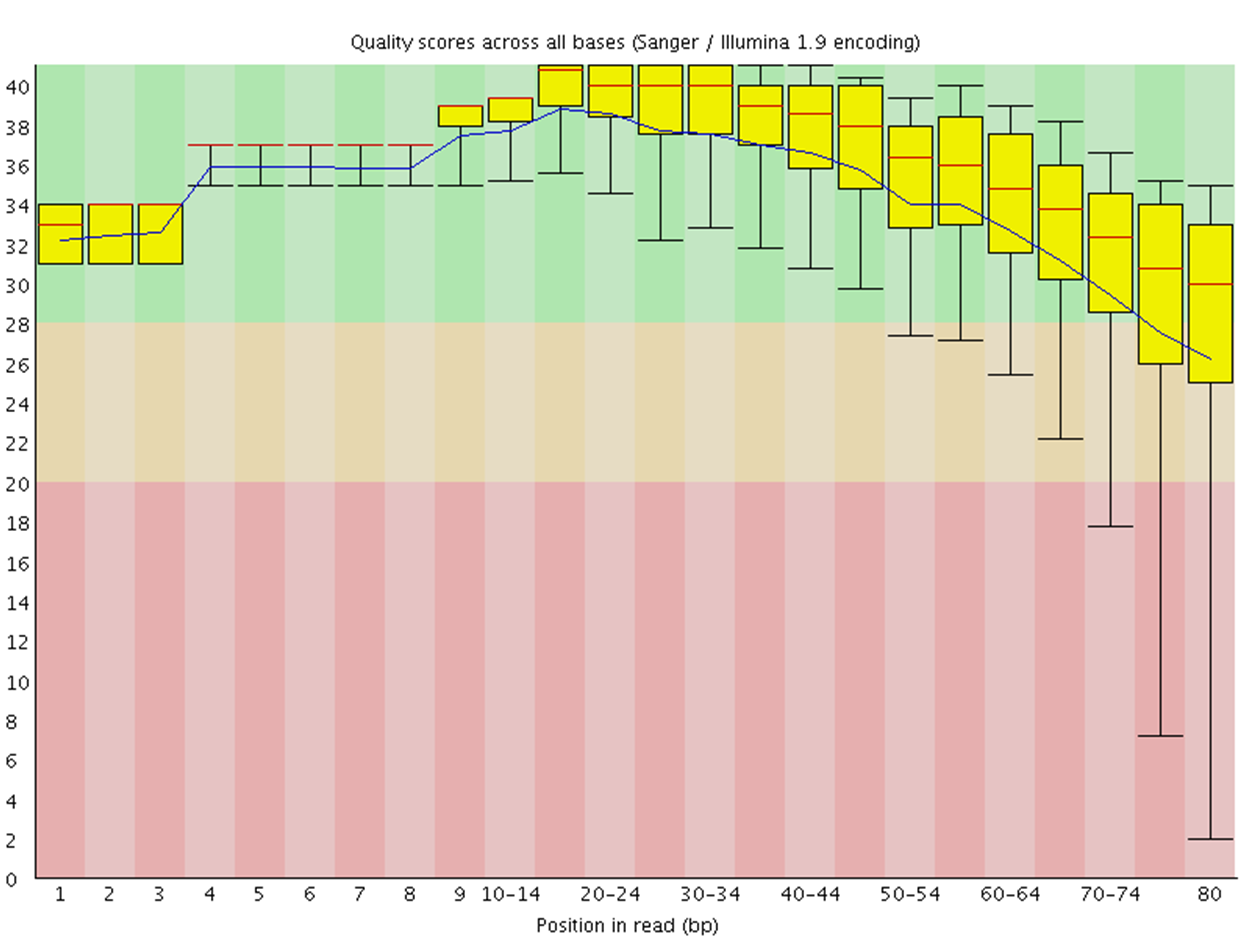
\includegraphics[width=0.8\textwidth]{ngs-qc/bad_example_trimmed_to_80bp.png}
\caption{per base sequence quality plot: visual output from FastQC. Base positions in the reads are shown on x-axis and quality score (Q Score) are shown on the Y-axis}
\label{fig:bad_example_trimmed_plot}
\end{figure}

\end{steps}

\subsection{Quality Based Trimming}
Base call quality scores can also be used for trimming sequence ends. A quality
score threshold and minimum read length after trimming can be used to remove low
quality data.

\begin{steps}
Run the following command to quality trim your data:
\begin{lstlisting}
cd ~/QC
fastq_quality_trimmer -h
fastq_quality_trimmer -Q 33 -t 20 -l 50 -i bad_example.fastq -o bad_example_quality_trimmed.fastq
\end{lstlisting}
\end{steps}

\begin{steps}
Run fastqc on the trimmed file and visualise the quality scores of the trimmed
file.

\begin{lstlisting}
fastqc -f fastq bad_example_quality_trimmed.fastq
firefox bad_example_quality_trimmed_fastqc/fastqc_report.html &
\end{lstlisting}

The output should look like:

\begin{table}[H]
  \centering
  \caption{FastQC Basic Statistics table}
    \begin{tabular}{ll}
    \toprule
    Filename & bad\_example\_quality\_trimmed.fastq \\
    \midrule
    File type & Conventional base calls \\
    Encoding & Sanger / Illumina 1.9 \\
    Total Sequences & 38976 \\
    Filtered Sequences & 0 \\
    Sequence length & 50-100 \\
    \%GC  & 48 \\
    \bottomrule
    \end{tabular}%
  \label{tab:badexamplequalitytrimmed}%
\end{table}%

\begin{figure}[H]
\centering
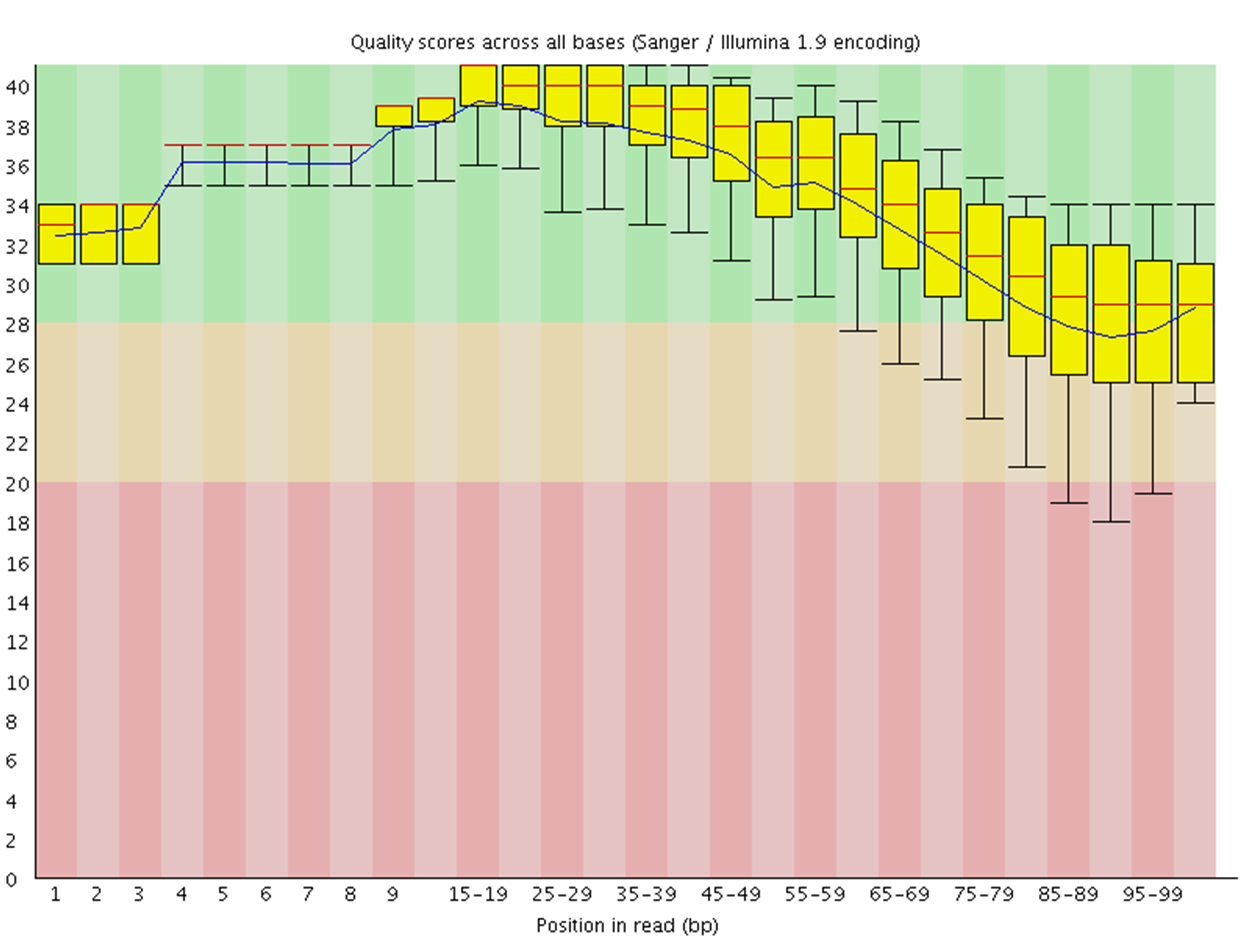
\includegraphics[width=0.8\textwidth]{ngs-qc/bad_example_quality_trimmed.png}
\caption{per base sequence quality plot: visual output from FastQC. Base positions in the reads are shown on x-axis and quality score (Q Score) are shown on the Y-axis}
\label{fig:bad_example_quality_trimmed_plot}
\end{figure}

\end{steps}

\begin{questions}
How did the quality score range change with two types of trimming?

Did the number of total reads change after two types of trimming?

What reads lengths were obtained after quality based trimming?

Did you observe adapter sequences in the data?

\end{questions}

\begin{advanced}
\subsection{Adapter Clipping}
Sometime sequence reads may end up getting the leftover of adapters and primers
used for the sequencing process. It's a good practice to screen your data for
these possible contaminations for more sensitive alignment and assembly based
analysis. This is usually a necessary steps in sequencing projects where read
lengths are longer than the molecule sequenced, for example when sequencing
miRNAs.

Various QC tools are available to screen and/or clip these adapter/primer
sequences from your data. (e.g. FastQC, fastx, cutadapt).

\begin{steps}
Here we are demonstrating \texttt{fastx\_clipper} to trim a given adapter
sequence.

\begin{lstlisting}
cd ~/QC
fastx_clipper -h
fastx_clipper -v -Q 33 -l 20 -M 15 -a GATCGGAAGAGCGGTTCAGCAGGAATGCCGAG -i bad_example.fastq -o bad_example_clipped.fastq
\end{lstlisting}
\end{steps}

\begin{note}
An alternative tool, not installed on this system, for adapter clipping is
\texttt{fastq-mcf}. A list of adapters is provided as a list in a text file. For more
information, see source URL on the front page of this tutorial.
\end{note}
\end{advanced}

\begin{advanced}
\subsection{Removing Duplicates}
Duplicate reads are the ones having the same start and end coordinates. This
may be the result of technical duplication (too many PCR cycles), or
over-sequencing (very high fold coverage). It is very important to put the
duplication level in context of your experiment. For example, duplication level
in targeted or re-sequencing projects may mean different than in RNA-seq
experiments. In RNA-seq experiments oversequencing is usually necessary when
detecting the low expressed transcripts.

\begin{information}
The duplication level computed by FastQC is based on sequence identity at the
end of reads. Another tool, Picard, determines duplicates based on identical
start and end positions.

\textbf{Due to time limitation we are not going to cover Picard. However, we
provide the following for your information.}

Picard is a suite of tools for performing many common tasks with SAM/BAM format
files. For more information see the Picard website and information about the
various command-line tools available:

\url{http://picard.sourceforge.net/command-line-overview.shtml}
\end{information}

\begin{information}
Picard 1.69 is installed on this system in \texttt{/usr/share/java/picard-1.69/}

One of the Picard tool (MarkDuplicates) can be used to analyse and remove
duplicates from the raw sequence data. The input for Picard is a sorted
alignment file in .bam format. Short read aligners such as, bowtie, BWA, tophat
etc. can be used to align fastq files against a reference genome to generate
SAM/BAM alignment format.
\end{information}

\begin{steps}
However interested users can use the following general command to run the
MarkDuplicates tool at their leisure and only need to provide a BAM file for the
INPUT argument:

\begin{lstlisting}
cd ~/QC
java -jar /usr/share/java/picard/MarkDuplicates.jar INPUT=<alignment_file.bam> VALIDATION_STRINGENCY=LENIENT OUTPUT=alignment_file.dup METRICS_FILE=alignment_file.matric ASSUME_SORTED=true REMOVE_DUPLICATES=true

\end{lstlisting}
\end{steps}

\end{advanced}

\chapterstyle{workshop}